\documentclass[12pt]{article}
\usepackage{geometry} % Pour passer au format A4
\geometry{hmargin=1cm, vmargin=1cm} % 

% Page et encodage
\usepackage[T1]{fontenc} % Use 8-bit encoding that has 256 glyphs
\usepackage[english,french]{babel} % Français et anglais
\usepackage[utf8]{inputenc} 

\usepackage{lmodern}
\setlength\parindent{0pt}

% Graphiques
\usepackage{graphicx,float,grffile}

% Maths et divers
\usepackage{amsmath,amsfonts,amssymb,amsthm,verbatim}
\usepackage{multicol,enumitem,url,eurosym,gensymb}

% Sections
\usepackage{sectsty} % Allows customizing section commands
\allsectionsfont{\centering \normalfont\scshape}

% Tête et pied de page

\usepackage{fancyhdr} 
\pagestyle{fancyplain} 

\fancyhead{} % No page header
\fancyfoot{}

\renewcommand{\headrulewidth}{0pt} % Remove header underlines
\renewcommand{\footrulewidth}{0pt} % Remove footer underlines

\newcommand{\horrule}[1]{\rule{\linewidth}{#1}} % Create horizontal rule command with 1 argument of height

%----------------------------------------------------------------------------------------
%   Début du document
%----------------------------------------------------------------------------------------

\begin{document}

\setlength{\columnseprule}{1pt}

\section*{Équation de Navier-Stokes}

L'équation de Navier Stokes permet de prédire la météo, de comprendre les océans, les cours d'air et cours d'eau... On étudie la \textbf{turbulence}.

On sait décrire son équation : 

$$\rho \left({\dfrac {\partial e}{\partial t}}+\mathbf {V} \cdot \mathbf {\nabla } e\right)={\mathsf {P}}:\mathbf {\nabla } \mathbf {V} +\mathbf {\nabla } \cdot \mathbf {q} +\mathbf {\nabla } \cdot \mathbf {q} _{R}.$$

Mais on ne sait pas la résoudre.

\subsection*{Problème du millénaire}

La résolution des équations de Navier-Stokes est un problèmes du millénaire. Si vous trouvez la solution, vous gagnez $1 \, 000 \, 000\$ $. 

  \begin{figure}[H]
        \centering
        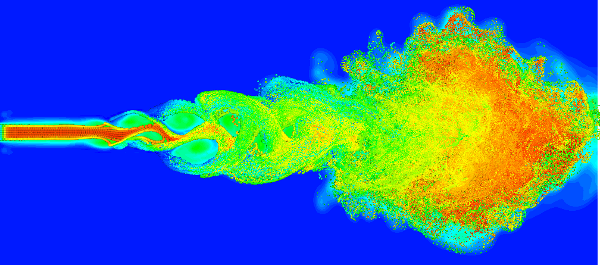
\includegraphics[width=0.6\linewidth]{4x5-calcul-litteral-1/sources/ns-1.png}
  \end{figure}

\begin{multicols}{2}

  \begin{figure}[H]
        \centering
        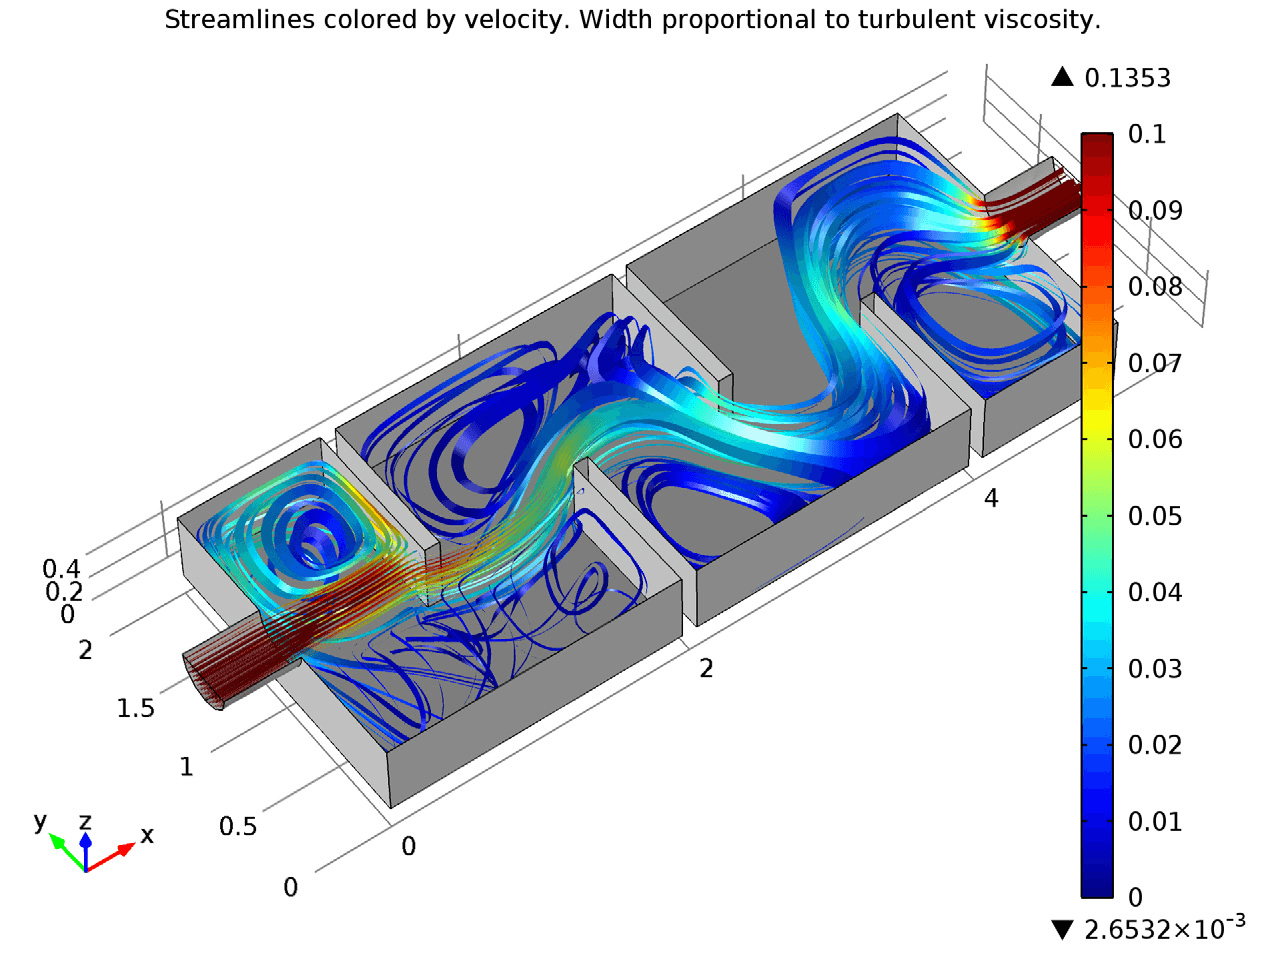
\includegraphics[width=0.8\linewidth]{4x5-calcul-litteral-1/sources/ns-2.png}
  \end{figure}
    \begin{figure}[H]
        \centering
        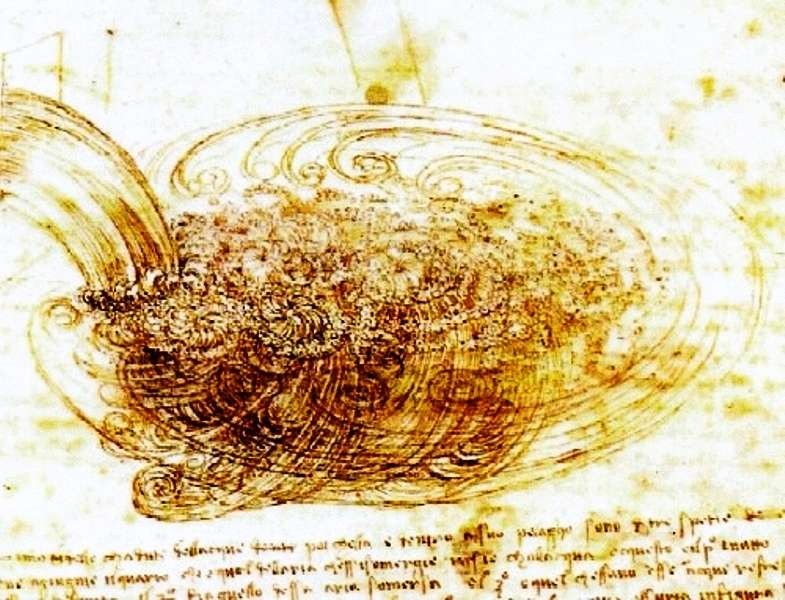
\includegraphics[width=0.8\linewidth]{4x5-calcul-litteral-1/sources/ns-3.png}
  \end{figure}

\end{multicols}

\begin{multicols}{2}

    \begin{figure}[H]
        \centering
        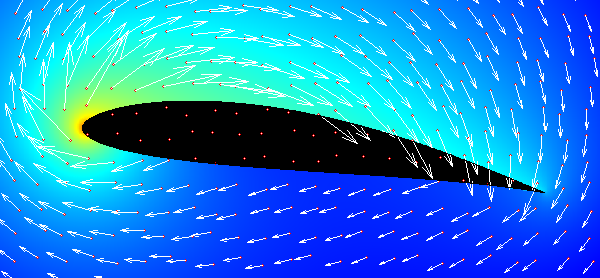
\includegraphics[width=0.8\linewidth]{4x5-calcul-litteral-1/sources/ns-4.png}
  \end{figure}

    \begin{figure}[H]
        \centering
        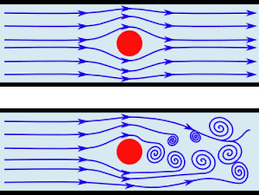
\includegraphics[width=0.8\linewidth]{4x5-calcul-litteral-1/sources/ns-5.png}
  \end{figure}
\end{multicols}

\end{document}